\documentclass{kththesis}


%Taken from ID1354
\usepackage[utf8]{inputenc}
\usepackage[english]{babel}
\usepackage{graphicx}
\usepackage{lastpage}
\usepackage{pgf}
\usepackage{wrapfig}
\usepackage{fancyvrb}
\usepackage{fancyhdr}
\pagestyle{fancy}
\usepackage{dingbat}
\usepackage{algpseudocode}
\usepackage{algorithm}
\usepackage{amssymb}

\usepackage[autostyle]{csquotes}
\usepackage[
    backend=biber,
    style=ieee,
    sortlocale=de_DE,
    natbib=true,
    url=true,
    doi=true,
    eprint=false
]{biblatex}
\addbibresource{references.bib}

\usepackage[]{hyperref}
\hypersetup{
    colorlinks=true,
}

% List of abbreviations
\usepackage{glossaries}
\makeglossaries

\title{Extending Timing Analysis for Non-Preemptive Task Sets on Multicore Under the AER Model}
\alttitle{Detta är den svenska översättningen av titeln}
\author{Jacob Kimblad}
\email{jacobki@kth.se}
\supervisor{Matthias Becker}
\examiner{Zhonghai Lu}
\programme{Master's Programme in Embedded Systems}
\school{School of Electrical Engineering and Computer Science}
\date{\today}


\begin{document}

%Term definitions
\newacronym{os}{OS}{Operating System}
\newacronym{cpu}{CPU}{Central Processing Unit}
\newacronym{lcu}{LCU}{Central Processing Unit}
\newacronym{aer}{AER}{Acquisition Execution Restitution}
\newacronym{cots}{COTS}{Commercial Off The Shelf}
\newacronym{edf}{EDF}{Earliest Deadline First}
\newacronym{rms}{RMS}{Rate-Monotonic Scheduling}
\newacronym{lcm}{LCM}{Least Common Multiple}
\newacronym{bcet}{BCET}{Best-Case Execution Time}
\newacronym{wcet}{WCET}{Worst-Case Execution Time}
\newacronym{prem}{PREM}{Predictable Execution Model}
\newacronym{gprem}{gPREM}{global \acrshort{PREM}}
\newacronym{ilp}{ILP}{Integer Linear Programming}
\newacronym{dms}{DMS}{Deadline Monotonic Scheduling}
\newacronym{ecu}{ECU}{Electronic Control Unit}
\newacronym{iip}{IIP}{Idle-time Insertion Policy}
\newacronym{a}{A}{Acquisition}
\newacronym{e}{E}{Execution}
\newacronym{r}{R}{Restitution}
\newacronym{csv}{CSV}{Comma-separated values}
\newacronym{autosar}{AUTOSAR}{Automotive Open System Architecture}
\newacronym{ip}{IP}{Intellectual Property}
\newacronym{np}{NP}{Non-Preemptive}
\newacronym{dag}{DAG}{Directed Acyclic Graph}
\newacronym{hulp}{HULP}{High-Utilization-Low-Period}
\newacronym{huhp}{HUHP}{High-Utilization-High-Period}
\newacronym{lulp}{LULP}{Low-Utilization-Low-Period}
\newacronym{luhp}{LUHP}{Low-Utilization-High-Period}
\newacronym{lu}{LU}{Low-Utilization}
\newacronym{hu}{HU}{High-Utilization}
\newacronym{rm}{RM}{Rate-Monotonic}
\newacronym{p-rm}{P-RM}{Precatious-\acrshort{rm}}
\newacronym{cw-edf}{CW-EDF}{Critical-Window-\acrshort{edf}}
\newacronym{us}{US}{United States}
\newacronym{can}{CAN}{Controller Area Network}
\newacronym{ecu}{ECU}{Electronic Control Unit}


% Frontmatter includes the title page, abstracts and table-of-contents
\frontmatter

\titlepage

\begin{abstract} 

    English abstract goes here.

\end{abstract}


\begin{otherlanguage}{Swedish} 
    
    \begin{abstract}

    \end{abstract} 

\end{otherlanguage}

% List of Acronyms
\printglossary[title={Acronyms}]

% Table of contents
\tableofcontents

% Mainmatter is where the actual contents of the thesis goes
\mainmatter


\chapter{Introduction and background} 


    %state the general topic and give some background


    %Start background here and have an even more general introduction?

Requirements on analysis and testing of systems in the automotive industry become of a bigger
concern with the rise of autonomous vehicles and the scepticism of their abilities to make
life-saving choices. Due to this research has been focusing on developing safer models that are
easier to test and are more deterministic within different areas of the vehicle. One such area is
the access to shared memory by different computers on the car. As modern cars can contain over 100
different processors, known as \acrshort{ecu}'s, internal communication between them is a
necessity. Communication is often done using some type of databus technology such as a
\acrshort{can}-bus. Sometimes a single \acrshort{ecu} can hold more than a single processing unit
(core) making it multi-core. Communication is then not only necessary between \acrshort{ecu}'s but
also internally between cores on a single \acrshort{ecu}. This is done through shared memory in a
non-deterministic way where all cores contest the access to memory creating congestion.

    %provide a review of the literature related to the topic

As an attempt to battle the problem of non-deterministic memory-access the \acrshort{aer}-model has
been proposed by \textcite{durrieu_predictable_2014} for use in the avionics industry. This model
proposes a new way of scheduling programs on processing cores to completely avoid memory
congestion, making the system easier more deterministic and easier to validate through testing. The
\acrshort{aer}-model already fits how existing programs are executed under the \acrshort{autosar}
standard for the automotive industry making the model a great candidate for further exploration into
its applicability.

    %define the terms and scope of the topic

The \acrshort{aer}-model divides each executed task up into three distinct parts, the
\acrfull{a}-phase, \acrfull{e}-phase and \acrfull{r}-phase. During the \acrshort{a}-phase the task
reads from shared memory and during the \acrshort{r}-phase the task writes to shared memory. The
\acrshort{e}-phase is strictly used for execution of the task and the task is not allowed to access
shared memory during this phase. Regular tasks are in opposite allowed to access shared memory
whenever they like, making the system less deterministic. However, knowing that the
\acrshort{aer}-model makes programs more deterministic is not sufficient to increase the safety. The
reason that deterministic programs is good is because they become much easier to analyse. However
changing how programs execute under new models often require different methods of analysis.

    %outline the current situation

Some analysis of memory-centric scheduling approaches exists such as the paper by
\textcite{alhammad_schedulability_2014} which explores analysis of an extension of the
\acrshort{prem} model on multi-core. Under \acrshort{prem} each task is divided into a computation
phase and memory phase. This is to be compared to the three-phase model \acrshort{aer} but without
the write phase. The write phase of a task is instead incorporated into the read phase of the task
running directly after on the same core as the first task creating the memory phase. In this way the
memory phase can further be divided internally into what the authors refer to as the pre-fetch and
write-back phases. The authors state the reason for only using two phases is that adding a write
phase would make analysis much harder for tasks that are dynamically scheduled. Another paper
written by \textcite{maia_schedulability_2017} focuses on improving the findings in the first paper
by creating analysis for the \acrshort{aer}-model from a memory-centric approach which reduces the
problem to single-core analysis which is an easier problem to solve than multi-core analysis.

    %evaluate the current situation (advantages/ disadvantages) and identify the gap

The existing research does have its shortcomings that could be improved. Since taking a
memory-centric approach to the problem also reduces it to a single-core problem it opens the
possibility to adapt existing analysis tools that are less pessimistic and scales better to larger
task amounts in their approach. One analysis tool proposed by \textcite{nasri_exact_2017} has shown
promising results for regular single-core scheduling analysis. This analysis is however not
available for \acrshort{aer}-modeled tasks and therefor would need to be adapted.

    %identify the importance of the proposed research



    %state the research problem/ questions

    %state the research aims and/or research objectives

    %state the hypotheses

    %outline the order of information in the thesis

    %outline the methodology


%With the increasing popularity of exploration into the capabilities of autonomous vehicles and 

%Embedded systems in the automotive sector are required to go through a lot of analysis and testing
%before being deemed safe for use in traffic. With the rise of autonomous vehicles these systems are
%becoming more complex as an effect of more computing needed being done. This has also put
%requirements on the hardware to become faster and faster, thus the industry is turning to the use of
%multi-core and many-core platforms. These type of platforms present more unpredictability than
%single-core platforms which requires new methods of analysis and deterministic execution of these
%systems. 


%\section{Background} 

%Timing analysis is an important part of real-time systems. However, multi-core platforms often
%implement complicated memory hierarchies that make timing analysis a lot harder. One way to tackle
%this is to explicitly schedule the access to shared memory in cooperation with computational tasks
%in a well-defined way. This can improve analysis and is employed by industrial domains already where
%the execution of tasks can be divided up into three distinct parts, read-execute-write.


\section{Problem}

The problem is that scheduling-analysis is hard and needs to be customized for many different ways
of scheduling tasks. Analysing embedded systems is hard but very necessary, especially hard are
multi-core systems that have complicated memory-hierarchies where cores share access creating
congestion. An emerging and already adopted technology to deal with it is to explicitly schedule the
access to shared memory using something like the \acrshort{aer}-model. Although some techniques does
exist to analyse scheduling under the \acrshort{aer}-model they are either not complete,
pessimistic or only allow for task-level priorities. Good analysis methods do exist for regular
tasks and can be adapted for the \acrshort{aer} model which is the problem this thesis searches to
solve.

%An analysis method for resource contention in multi-core real-time systems have been proposed in
%paper. This analysis method is however not customised for the read-execute-write execution model
%that is adapted both within the avionics domain and automotive domain.


\section{Purpose}

The purpose of the thesis is to expand an existing analysis method by adding to the source code and
produce a version of the \acrshort{aer}-model that is compatible with the analysis method and to
evaluate the characteristics of the model when changing different input variables in the tasks.

%The purpose is to expand existing analysis methods by adding to the source code and/or produce a
%model of the read-execute-write task model that is available as input for these formal analysis
%methods.

\section{Goals}

The goals of the project can be summarized into the following key points.

\begin{itemize}
    \item Perform a state-of-the-art literature study within the research area.
    \item Generate task-sets in a fair way.
    \item Transform the tasks into appropriate input to the analysis tool.
    \item Extend the analysis tool to handle the \acrshort{aer}-model.
    \item Present a customisation to the \acrshort{aer}-model for better compatibility with the analysis tool.
    \item Present an evaluation to the analysis tool after extension through benchmarking.
\end{itemize}


\subsection{Benefits, Ethics and Sustainability}

Benefits of this thesis includes trying to make time-critical systems that exist within systems such
as airplanes and cars more deterministic. More deterministic system is easier to analyze and test
for faulty behaviour, which leads to less system failures that may be a cause of human harm. As
increasing safety of these systems leads to less unnecessary harm being caused to humans which is
beneficial to society it logically follows through deductive reasoning that the thesis is
beneficial.

As the projects focus is on avionics and automotive sector which is the largest contributor to
greenhouse grass emission within the \acrshort{us} totaling at 29\% of all emissions during
2017\parencite{us_epa_inventory_2017} it does raise some ethical concerns as to whether this is
something the thesis contributes to and if in that case there are more sustainable alternatives.

\section{Methodology / Methods}

%TODO: How are these things used in practice? Is this section required?
The theoretical research methods and methodologies have been chosen following the guidelines
presented in \textcite{hakansson_portal_2013}. The thesis will take a quantitative research approach
to try and refute or verify the presented theories. Experimental research methods will be applied
under the fundamental philosophical assumption of positivism where facts and truths about the world
is assumed to be gathered through our sensory experiences. A deductive research approach is used
where data is analyzed to see if the theories can be supported or not. To gather the data an
experimental research strategy will be used where all factors and variables that can affect the
experiment are controlled for to create large data sets that can be analyzed using statistical data
analysis methods. The data must then be assured to be reliable, valid and replicable to ensure that
the conclusions made from it is correct.


\section{Delimitations}

Only covers a special case of the \acrshort{aer}-model presented in section
\ref{sec:work_task_model} where the acquisition- and restitution-phases both have dedicated windows
as parts of the total scheduling window within which they are allowed to execute. Due to the novelty
of the research there is no other scheduling analysis tool that can be used in order to find a
comparison of how well it performs. However, since the analysis tool is exact we can expect that
other analysis tools will either perform the same (being also exact) or worse.


\section{Outline}

Chapter \ref{ch:theoretic_background} gives a theoretic background to the problem area such that the
reader becomes equipped to understand the topic at hand in-depth.

%We use the \emph{biblatex} package to handle our references.  We therefore use the command
%\texttt{parencite} to get a reference in parenthesis, like this \parencite{heisenberg2015}.  It is
%also possible to include the author as part of the sentence using \texttt{textcite}, like talking
%about the work of \textcite{einstein2016}.

\chapter{<Theoretic Background> Use a self-explaining title}\label{ch:theoretic_background}

This chapter aims to give sufficient background such that the reader is able to understand the work
that the thesis covers. Section \ref{sec:the_task_model} begins by describing the task model used
within embedded systems.


\section{The Task Model} \label{sec:the_task_model}

%TODO: Maybe add a picture that shows all the characteristics of a job/task
%TODO: Show that this is something that can actually be used in AUTOSAR as they already to the
%fetch-execute-write cycle for some of their streaming applications using runnables. Called
%"implicit access" in autosar. Depicted in Real World Automotive Benchmarks for Free pp-slides.
A periodic task, denoted as $\tau_i$, is a unit of work that is executed periodically on a processor
alongside other tasks over and over again. In embedded systems a task is usually completed in some
amount of time known as its \textbf{computation time}, denoted as $C_i$. Once a task has finished
executing it will usually wait for some amount of time before it is ready to execute again, this is
known as the tasks \textbf{period}, denoted by $T_i$. The earliest time where a task is ready to
start execution within a new period is called the \textbf{arrival time} of the task and is denoted $
a_i $. Note that the arrival time is equal to the beginning of the current period of the task.

The \acrshort{lcm} of the periods for all the tasks in a task set is known as the task set's
\textbf{hyper-period} and is an important concept in scheduling tasks which is further discussed
in section \ref{sec:scheduling}. The hyper-period is defined as $H = \acrshort{lcm}(P_i)$ for $i =
1, 2, ..., n$. Each task is also required to finish execution before a set amount of time starting
from each new period belonging to the specific task, this is known as the task's \textbf{relative
deadline} denoted as $D_i$. For an \acrshort{os} to decide in what order the tasks should execute
when more than one is available at the same time they are each assigned a \textbf{priority}, denoted
by $P_i$, by a scheduler which is further discussed in section \ref{sec:scheduling}. A task can thus
be introduced by defining its characteristics as $\tau_i = (C_i, T_i, D_i)$. It is then also possible to
define a task set as $ \Gamma = \{\tau_1, \tau_2, \tau_3, ..., \tau_n\} $. In the case where the
execution time of the task is defined as a member in the interval from the \acrshort{wcet} to the
\acrshort{bcet} as such $C_i \in [C_i^{min}, C_i^{max}]$ the task can instead be defined as $\tau_i
= ([C_i^{min}, C_i^{max}], T_i, D_i)$.

Following the above definitions state can be can ascribed to tasks depending on their status in the
system at a specific time instance. A task is in the \textit{ready} state when it still needs time
to complete its execution before its deadline but is not yet allowed access to the processor. Once a
task is moved out of the ready state and is executing on the \acrshort{cpu} it is said that the task
is \textit{running}. The task can also be moved back to the ready state from running state before
execution is finished by being \textbf{preempted} by the scheduler. If a task requires access to
some shared resource that is not currently available, thus halting execution, the task is said to be
\textit{waiting}. Once the shared resource is available again the task is moved back into the ready
state. The three different states and their transitioning are depicted in figure
\ref{fig:ready_running_blocked_model}.

\begin{figure}

    \centering

    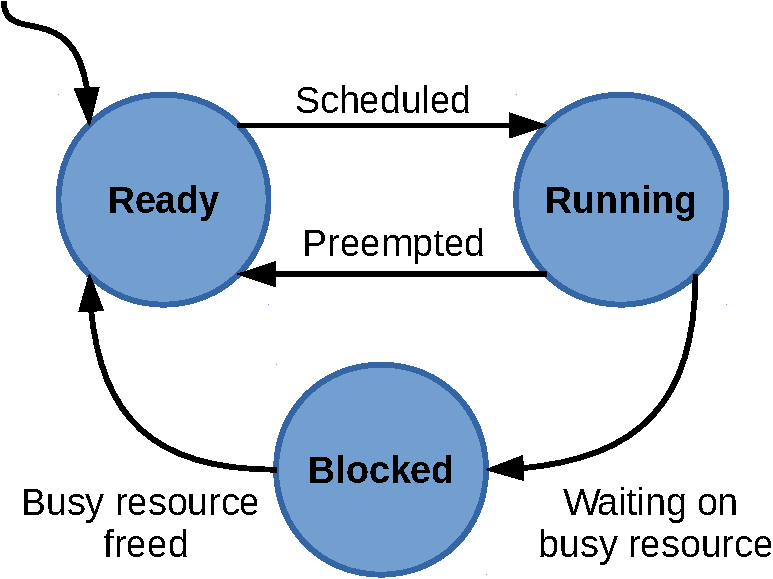
\includegraphics[width=0.7\linewidth]{images/ready-running-blocked-model.pdf}

    \caption{The three states a task may be in.}

    \label{fig:ready_running_blocked_model}

\end{figure}

The task model presented thus far has made some assumptions that are not realistic, such as the
release time and computation time being exactly the same each period. In order for the model to
better represent reality to increase the validity of schedulability analysis methods some additional
concepts are introduced. Computation time of a task varies because of unpredictable behaviour in the
processor such as caches. Therefor the notions of \acrfull{bcet} and \acrfull{wcet} is introduced to
represent the interval between the fastest and the slowest computation time of a specific task.  To
denote this $ C_i^{min} $ and $ C_i^{max} $ is used. In addition to uncertainties in the computation
time there are also uncertainties in the arrival time of tasks. The notion of earliest arrival time,
denoted $ a_i^{min} $, is the  absolute earliest time at which a task may be able to start executing
within the period and likewise the latest arrival time, denoted $ a_i~{max} $ is the time when the
task is guaranteed to be able to start execution. In addition, the intervals for computation times
and release jitter can be represented as a probability distribution, but this will not be covered in
this thesis.


% TODO: Introduce the notion of offline and online schedulers, start time of tasks (when they start
% execution)
% TODO: Mention Job-Level priority (JLP) and Task-Level Priority (TLP)
\section{Scheduling} \label{sec:scheduling}

Although computers give away the illusion of being able to deal with many things simultaneously this
is actually not the case. Computers are limited to how much parallel computing they are able to do
by the hardware, specifically the amount of cores within the \acrshort{cpu}. A computer with, for
example, a single core \acrshort{cpu} is only able to execute one task at a time. For a computer
with a single core to deal with more than a single task at the same time requires switching ongoing
tasks in and out of the core during runtime. For the \acrshort{os} to switch tasks quickly in and
out of the core it needs to schedule the tasks according to some order. This is where the priority
of tasks come in handy, by scheduling tasks and switching them in and out of the processor very
quickly depending on their priority the \acrshort{os} is able to perform more than one task seemingly in
parallel than what is actually allowed for by hardware. The rest of this section up until section
\ref{subsec:multiprocessor_scheduling} is only concerned with the scheduling of single core
processors.

% TODO Maybe add other measurements of how good schedulers are, least-slack time etc.
The order in which tasks are executed is determined by the scheduler which in of itself is a special
type of task executed by the \acrshort{os}. The scheduler is invoked by specific events happening in
the system. It could for example be that a task is finished executing or that it has begun waiting
on some resource that is not yet available. As not all scheduling algorithms were created equal they
vary in how good of a task they do when scheduling the same task sets. Because of this some
measurements must be introduced in order to have a fair comparison of how well they work. The
processor utilization factor, denoted as $ U $, is such a measurement introduced to show to what
percentage a specific task set would keep the processor busy. The utilization can be calculated as
$ U = \sum_{i=1}^n \frac{C_i}{T_i} $.

For embedded systems there exists a set of well known scheduling algorithms such as \acrshort{edf}
and \acrshort{rms}. Imagining a single-core \acrshort{cpu} the algorithm \acrshort{rms} works by
setting the priority of each task equals to its period. This means that the task with the lowest
period is given the highest priority and always scheduled first once it is in the ready state. Since
periods of tasks never changes during execution, the priorities of the individual tasks will never
change either, thus \acrshort{rms} is said to be a \textbf{static-priority scheduler}. If a
scheduler instead changes the priorities of the task during execution it is a
\textbf{dynamic-priority scheduler}. 

Instead of setting priorities according to the periods, \acrshort{edf} works by setting the
priorities according to how close a task is to its deadline. This means that the task closest to
exceeding its deadline will always be executing first on the processor. If some task $ \tau_a $ is
executing with a deadline further away in time than another task $ \tau_b $, that was just released,
then $ \tau_a $ will get preempted and the newly released $ \tau_b $ will be allowed to execute
instead. This behaviour makes \acrshort{edf} a \textbf{preemptive scheduling algorithm}, the
opposite of which is a \textbf{non-preemptive scheduling algorithm} which lets each task finish
before scheduling the next highest priority task.

An example of how \acrshort{rms} would schedule a task set can be seen in figure
\ref{fig:rate_monotonic_scheduling}. A special point of interest is at time 4 when $T_3$ is
executing since earlier as $T_1$ is released. Due to $T_1$ having a lower period than $T_3$ it also
has a higher priority. The scheduler preempts $T_3$ and lets $T_1$ execute instead. $T_3$ is later
allowed to resume execution of $j_3$ at time 5.

\begin{figure}

    \centering

    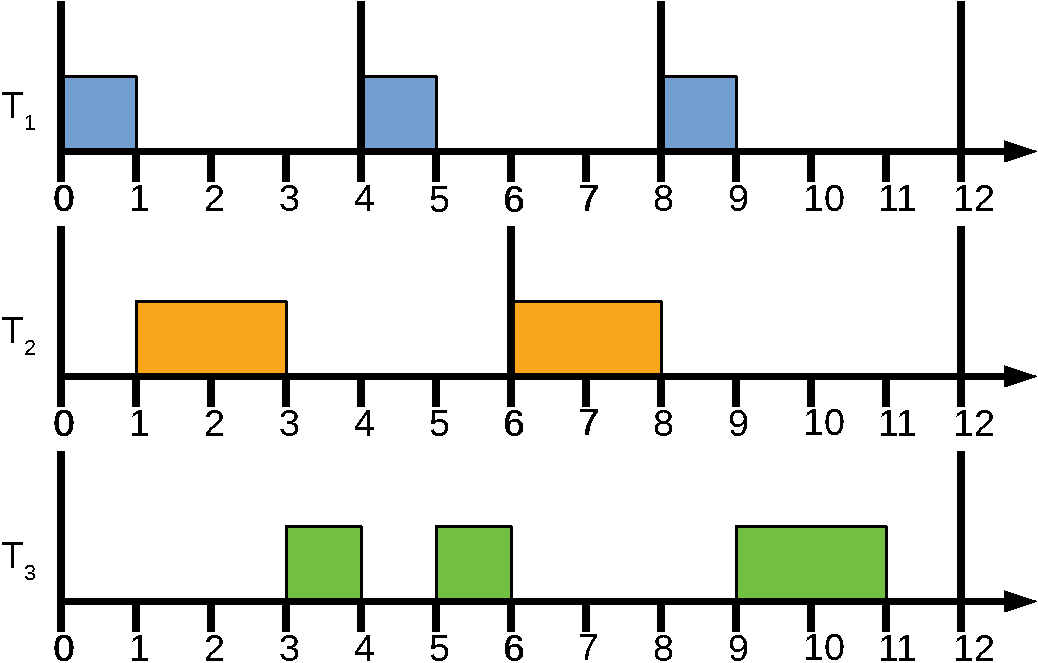
\includegraphics[width=0.8\linewidth]{images/rate-monotonic-scheduling.pdf}

    \caption{Example of rate monotonic scheduling for three tasks where $T_1=(1, 4, 4)$, $T_2=(2, 6,
    6)$, $T_3=(4, 12, 12)$.}

    \label{fig:rate_monotonic_scheduling}

\end{figure}

When dealing with non-preemptive single-core systems where the tasks periods equal the tasks
deadlines \acrshort{rms} guarantees finding a feasible schedule if such a schedule exists, making it
an \textbf{optimal} scheduling algorithm. For preemptive single-core systems, \acrshort{edf} has
been proven to always find a feasible schedule if one exists, making it optimal in those
circumstances. If an algorithm however is unable to find a feasible schedule, even when such a
schedule exists, it is considered a \textbf{heuristic}.

\subsection{Multiprocessor scheduling} \label{subsec:multiprocessor_scheduling}

When considering multi-core processors life for schedulers become a little harder. On a single-core
processor the scheduler only needs to consider temporal allocation of the task, as in
\underline{when} they should run. Scheduling tasks on a multi-core system also requires the
scheduler to consider spatial allocation of the tasks, as in \underline{where} they should run
(on what core). Schedulers deal with these allocations in two different ways, either through what is
known as \textbf{global scheduling} or through \textbf{partitioned scheduling}. 

%TODO: Mention some examples of multi-core scheduling algorithms (gEDF, RMS, etc)
%TODO: maybe have pros and cons for partitioned and global scheduling
%TODO: Maybe have a picture to help explain the differences between partitioned and global
%scheduling. This contains a good example:
%http://retis.sssup.it/~giorgio/slides/cbsd/mc3-global-2p.pdf
Partitioned scheduling entails that each task is assigned to a dedicated core where it always will
be running. Due to this any single-core scheduling algorithm can be used individually on each core
during runtime. It is then possible to also use the existing scheduling analysis methods for the
respective scheduling algorithm.  This sounds easy enough, but in reality assigning tasks to cores
is a version of the bin packing problem which is known to be a NP-hard problem meaning that there
exists no algorithm to solve it in less than polynomial time. However, good heuristics
\parencite{johnson_fast_1974}\parencite{coffman_application_1978} exists that find good solutions
fast and since tasks can be allocated to cores offline more computing power can be used to find
close to optimal solutions in reasonable time.

Global scheduling means that the scheduler takes into account both spatial and temporal allocation
when scheduling each task. Algorithms from sing-core scheduling can be applied to global scheduling
such as \acrshort{rms} and \acrshort{edf}, but they will have different behaviour. Global scheduling
decreases the determinism of the system and creates more combinations of possible schedules for each
task set.

\section{Schedulability analysis}

%TODO mention brute-forcing analysis by simulating one hyper period of the schedule. And this seems
%easy in theory, but in practice there can be hundreds of tasks and super long hyper period.
When developing new scheduling methods it is important to put the schedules that they produce under
analysis as to show whether they are feasible or not. It is especially important when the schedules
are used in hard real-time systems like those found in the avionics and the automotive sector where
missed deadlines could mean fatal outcome. For example, \acrshort{rms} can be analysed
mathematically and has been proven to be able to schedule any task set that fulfills the constraint
$ U \le n(2^{\frac{1}{n}}-1) $ where $ n $ is the amount of tasks \parencite{liu_scheduling_1973}.
This is only a \textbf{sufficient} condition, meaning that \acrshort{rms} might be able to schedule
task sets that do not fulfill the condition, but it is not guaranteed to. A condition that must be
fulfilled for the task set to have a feasible schedule, but does not guarantee such a schedule
exists, is known as a \textbf{necessary} condition. If a condition is both necessary and sufficient
it is said to be \textbf{exact}. An example of an exact condition for \acrshort{edf} is $ U(\Gamma)
\leq 1 $ which states that the utilization of the task set must be one or less. Finding good
conditions is not always trivial as shown by \parencite{bini_hyperbolic_2001} which presents a less
pessimistic sufficient condition of the same complexity $ O(n) $ for \acrshort{rms} almost 30 years
after the earlier presented condition was introduced. 

%TODO: Mention that increase of tasks leads to harder schedulability
%TODO: Mention that the illustration is mostly to get and idea of the problem trying to be solved,
%and that it represents single-core and a multi-core representation would look slightly different
%(due to a single task not being able to utilize all cores), but the idea is the same.
The gap between sufficient conditions and necessary conditions where the tasks sets are undetermined
if they are able to be scheduled is illustrated in figure
\ref{fig:sufficient_necessary_schedulability}. A lot of research is being aimed towards finding less
pessimistic necessary and sufficient conditions for multi-core scheduling algorithms to close the
gap between them which is still not a solved problem. In addition, each unique scheduling algorithm
may require its own set of unique conditions for analysis. All conditions are also not as simple as
the one presented for \acrshort{rms} especially when considering multi-core. The conditions have
varying complexity and they often need to make the trade-off between complexity and how pessimistic
they are. The paper \parencite{bertogna_tests_2011} shows examples of conditions that are of $
O(n^3) $ complexity which can be alright when analysing small task sets, but is too complex as the
task sets grow or if it has to be calculated online with limited computation power.

\begin{figure}

    \centering

    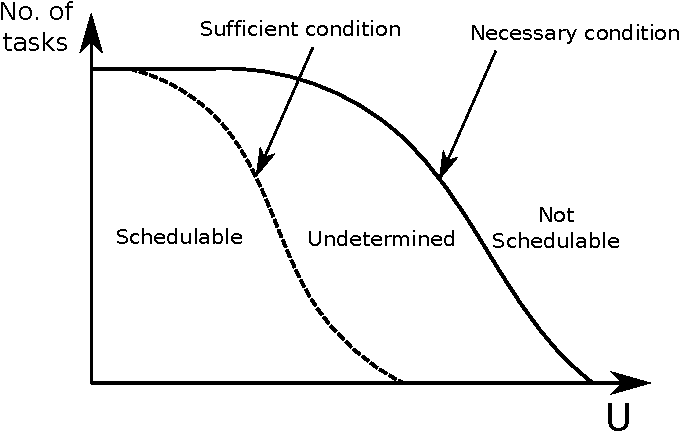
\includegraphics[width=0.8\linewidth]{images/sufficient_necessary_schedulability.pdf}

    \caption{Research aims to shrink the gap left between sufficient and necessary conditions.
    Illustration inspired by \parencite{sebestyen_simulation-based_2012}.}

    \label{fig:sufficient_necessary_schedulability}

\end{figure}

% TODO: Is this section really necessary? Perhaps preface with it by explaining there are different
% ways of analysis. Other than mathematically, we can also simulate the schedule and look for missed
% deadlines. Don't use the word simulation, we are only doing analysis, otherwise people will be MAD
% TODO: Critical instant is worst case for a specific task. Only for RMS and EDF is this when all higher
% prio tasks are released at the same time.
An example of a precise schedulability test for \acrshort{rms} on single-core systems is to find the
so called \textbf{critical instant} of a task. This is when all higher priority tasks are released
at the same time as the task. This pushes the task completion time as far away from its release time
as it ever will be in the given task set. If the task doesn't miss its deadline after the critical
instant it is guaranteed to never miss its deadline for any other instance in the schedule. As an
effect of this, each task can be examined during its critical instant, and if all tasks meet their
deadlines the task set is guaranteed to be schedulable. This facilitates analysis considerably as
only a small part of the schedule needs to be analysed.

Having the arrival and computation time defined as intervals creates the possibility of different
schedules for the same task set using the same scheduler. This makes analysis more difficult as
simulation requires testing several of the combinations of release and computation times. It is
intuitive to think that it is sufficient to analyse the worst-case times of all tasks to find if the
schedule is feasible. This is however not true for non-preemptive systems as two jobs released
within the same interval can lead to either being scheduled until its completion before the other.
For some task sets with this property an earlier release of a certain job can lead to a missed
deadline later in the schedule in multi-core systems. This also means that examining the critical
instant of a task is no longer sufficient in determining if a task set is schedulable or not.
% TODO Example of how earlier release of a task on multicore systems can make the schedule miss a
% deadline while a later release of the same task may have been able to complete the deadline.


\section{Non-Preemptive schedulability test}

The work which this thesis builds upon is presented in \parencite{nasri_exact_2017}. An open-source
implementation written in c++ by one of the authors is available on
Github\parencite{brandenburg_implementation_2018} and will further be referred to as the
\acrfull{np}-test. It presents an exact non-preemptive schedulability test for single-core
processors. The basic idea is to build a schedule graph that fully represents all possible schedules
for a given job-input. This isn't a new idea but it brings a novel merge phase that merges all nodes
of the graph that will lead to the same input in the future making it scale better. It also takes
into account uncertainties in the job set to better reflect reality by taking both release-time
jitter and the \acrshort{bcet} and \acrshort{wcet} into consideration. The test is both sufficient, 
necessary and sustainable. Where sustainable is defined as "A schedulability test is defined to
be sustainable if any task system deemed schedulable by the test remains so if it behaves 'better' than
mandated by its system specifications"\parencite{baruah_sustainable_2006}. Thus also making it exact.

The analysis tools is also able to deal with non-work-conserving schedulers by accepting an
\acrshort{iip} function. An \acrfull{iip} is used during scheduling to see if the highest priority
task is to be scheduled at the present time when there is a free core to schedule the task onto or
if the core should be left idle. The idea is that a non-work-conserving algorithm can increase
schedulability by trying to make smarter scheduling choices. Two existing \acrshort{iip}'s are
already implemented in the \acrshort{np}-test, the first one is \acrfull{p-rm}
\parencite{nasri_precautious-rm:_2014} and the second \acrfull{cw-edf}
\parencite{nasri_non-work-conserving_2016}.


The job-set containing 9 unique jobs derived from the tasks $\tau_1=([3,13], 60, 60)$, $\tau_2=([7,
8], 30, 30)$ and $\tau_3=([1,2], 10, 10)$, no release jitter is assumed, is presented in
\parencite{nasri_exact_2017}. These are scheduled according to figure \ref{fig:np-test_schedule}
when every job executes for its \acrshort{wcet} and the result is that they all meet their
deadlines. However, if $J_7$ would instead execute for one time unit less it would result in the
schedule depicted in figure \ref{fig:np-test_schedule_fail} where $J_2$ misses its deadline. This
example perfectly shows the problem with analysing \acrshort{np} scheduling as it is not sufficient
to just check if all deadlines are met when all jobs execute for their \acrshort{wcet}. The task-set
is shown to become feasible if the priorities are reordered as $ p_1 < p_2 < p_3 < p_4 < p_5 < p_5 <
p_9 < p_7 < p_8$.



\begin{figure}

    \centering

    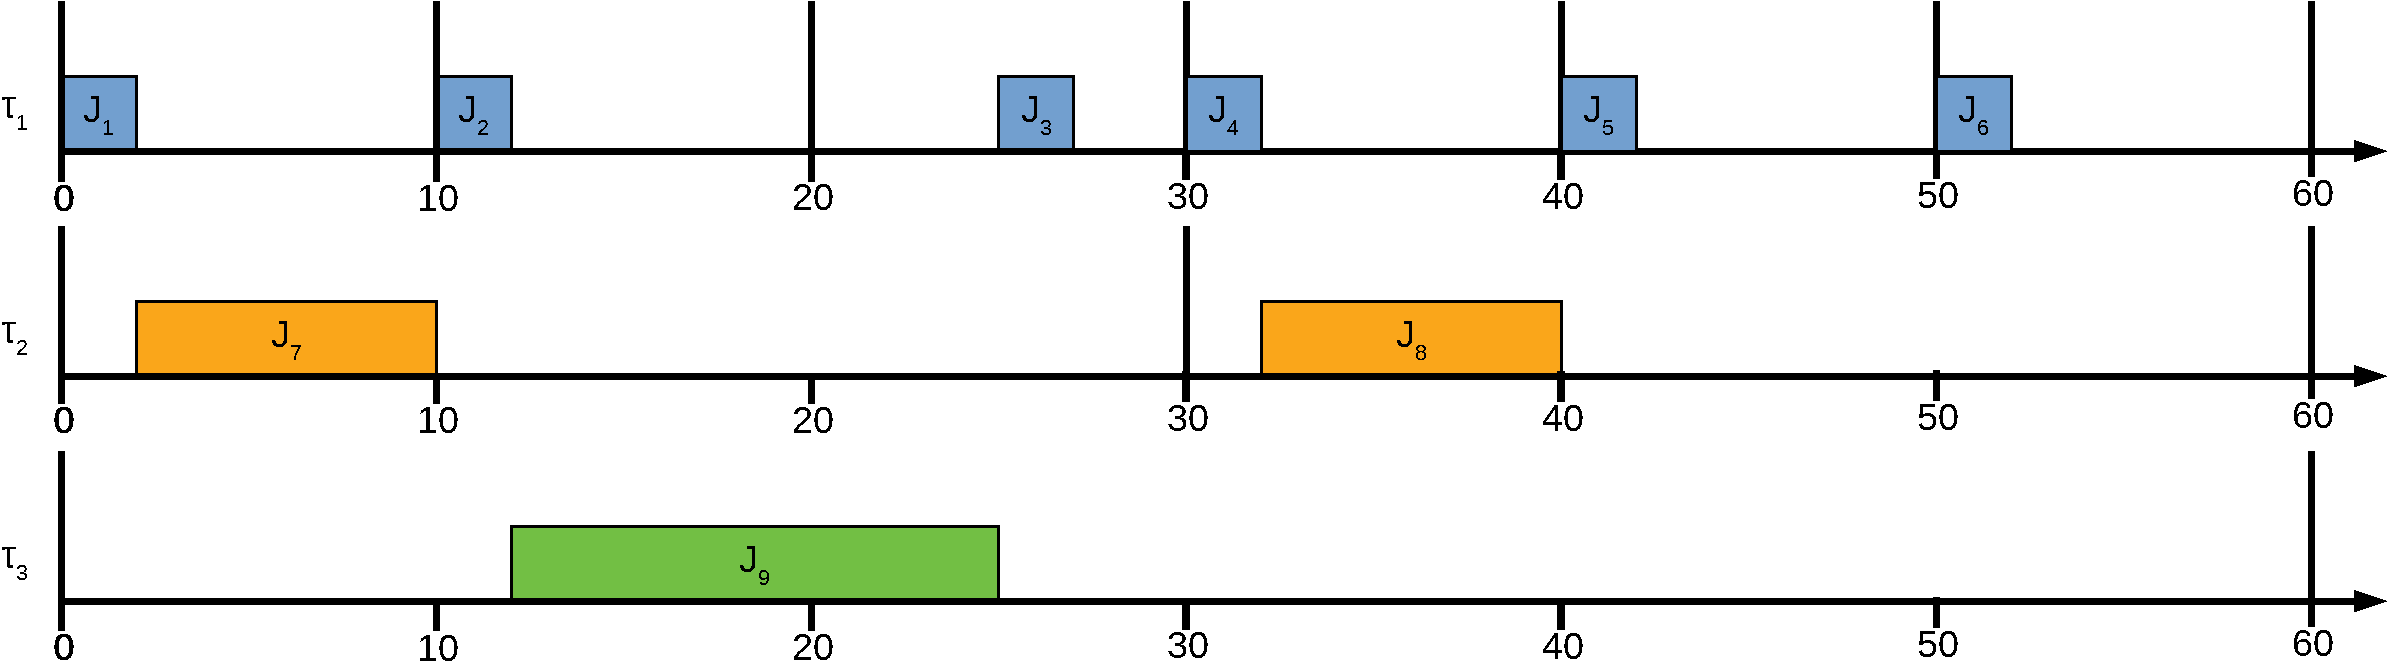
\includegraphics[width=1.0\linewidth]{images/np-test_schedule.pdf}

    \caption{Non-preemptive task-set scheduled under \acrshort{edf} or \acrshort{rms}}

    \label{fig:np-test_schedule}

\end{figure}


\begin{figure}

    \centering

    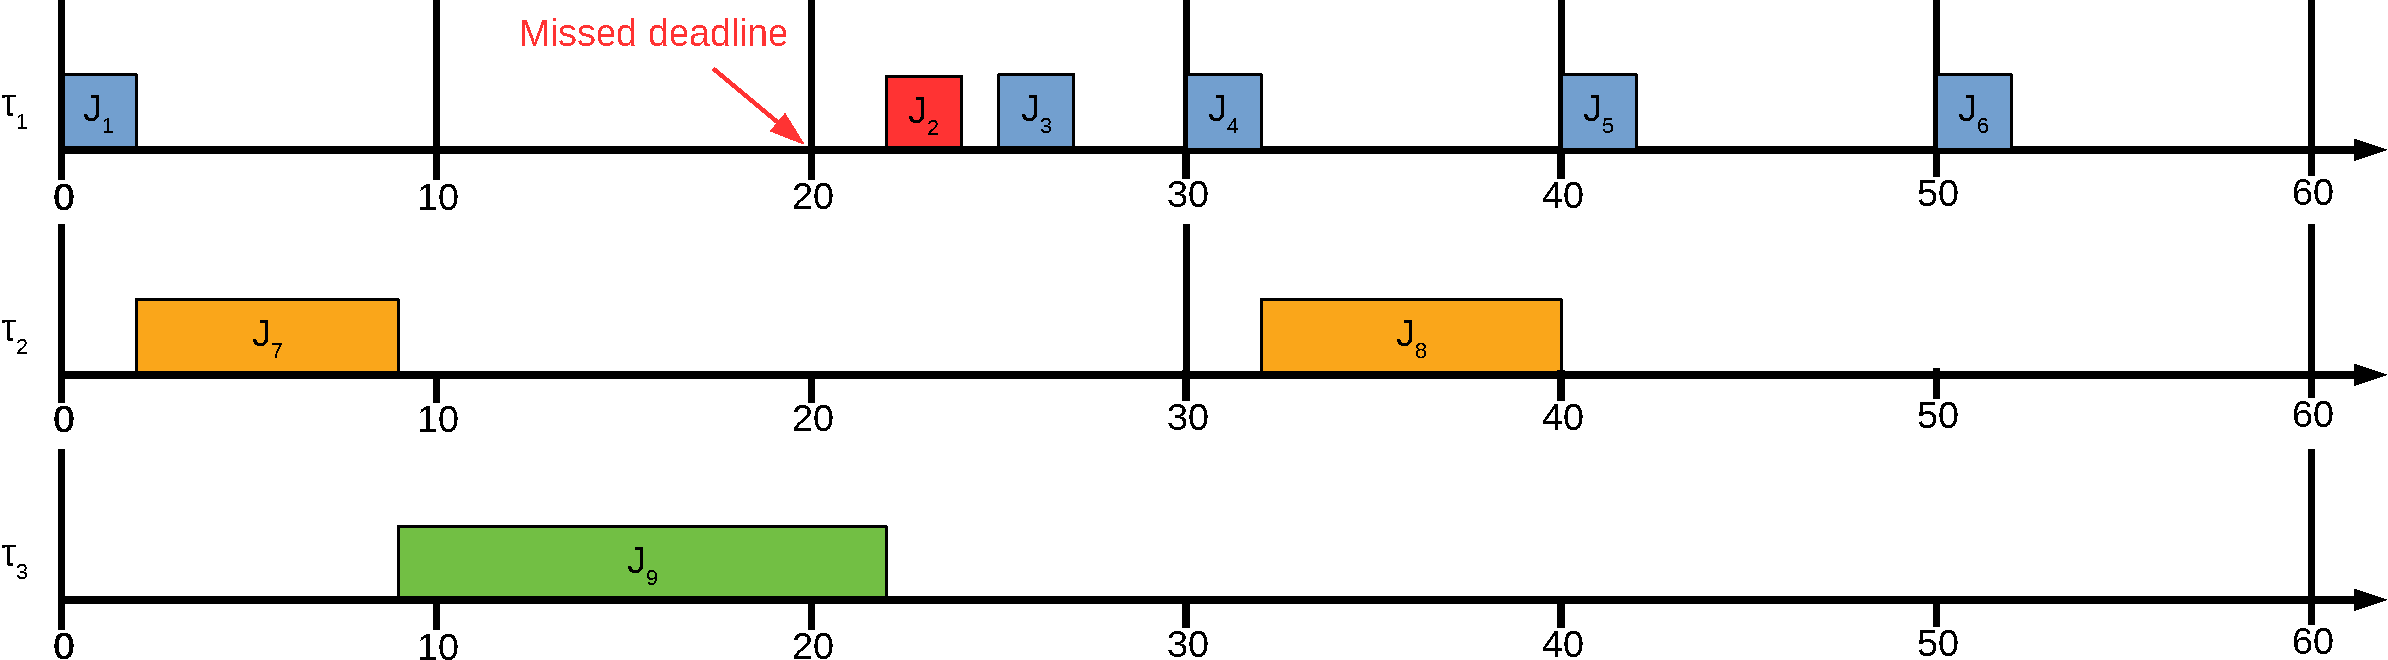
\includegraphics[width=1.0\linewidth]{images/np-test_schedule_fail.pdf}

    \caption{Non-preemptive task-set where $J_7$ finishes 1 time unit earlier, scheduled under
    \acrshort{edf} or \acrshort{rms}}

    \label{fig:np-test_schedule_fail}

\end{figure}


The scheduling graph is a \acrshort{dag} where each edge represents a scheduling decision and each
vertex represents a time-interval. The graph is built from the root node by making scheduling
decisions. Looking back at the previous job-set, part of its scheduling graph would be represented
by the \acrshort{dag} depicted in figure \ref{fig:scheduling_graph} when scheduled under
\acrshort{edf}. From the root vertex $v_1$ the highest-priority job of all available jobs is
scheduled, job $J_1$, and an edge is added to represent it. The other end of the edge is connected
to a new vertex $v_1$ that represents the interval within the scheduled jobs may finish execution
within. Since the \acrshort{wcet} is 2 and \acrshort{bcet} is 1 for $J_1$ the interval for the new
vertex is $[1, 2]$.  For all times within this interval the highest priority-job that has been
released is job $J_7$ and is thus scheduled.  Its \acrshort{wcet} is 8 and its \acrshort{bcet} is 7.
These are added to the interval of the possible finish times from the previous vertex and creates
the new interval $[8,10]$. Now as demonstrated in figures \ref{fig:np-test_schedule} and
\ref{fig:np-test_schedule_fail} there are two scheduling possibilities that are dependent on when
the previous jobs have finished execution. If $J_7$ finishes before time 10 then $J_9$ will be the
highest priority released job, and if $J_7$ finishes at time 10 then $J_2$ is the highest priority
released job. Since two different scheduling decisions can be made within the interval represented
by vertex $v_3$ two new edges are branched out from that vertex, each representing one of the two
scheduling decisions. If $J_2$ is scheduled it must start at time 10, to this is added its
\acrshort{wcet} 2 and \acrshort{bcet} 1 to create the interval represented by the vertex $v_5$. If
$J_9$ is scheduled it can start withing the interval $[8, 9]$, and thus its \acrshort{wcet} 13 and
\acrshort{bcet} 3 is added to that interval to create vertex $v_4$. At this point each of the two
branches continue scheduling jobs and branch out whenever several options are available until either
all jobs have been scheduled, or a job fails to meet its deadline as depicted in
\ref{fig:scheduling_graph}. This will for large job sets create a huge search space that is very
computation and memory intensive and does not scale very well. However, the novelty of the approach
presented in \parencite{nasri_exact_2017} is to introduce a merge-phase. The merge phase tries to
decrease the search space by merging vertices that lead to similar execution scenarios. The
criteria for merging two vertices is that (a) the same jobs have been scheduled before the vertices
and (b) the finish-time interval they both represent overlaps, i.e. $v_i \cap v_j \neq \emptyset$.
When this is the case the new vertex $v_n$ that is created from the merge represents the union of
finish times from the two merged vertices $v_i$ and $v_j$ as such $v_n \gets v_i \cup v_j$. Both of
these criteria are fulfilled for vertices $v_4$ and $v_5$ meaning that they can be merged into a
single vertex. The merging is illustrated in figure \ref{fig:scheduling_graph_merge} which also
shows the edges that no longer needs to be explored using dashed lines.


\begin{figure}

    \centering

    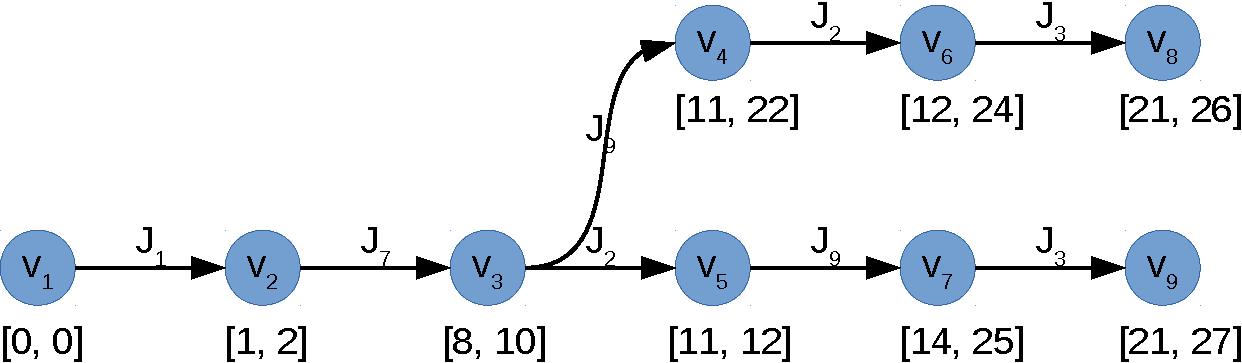
\includegraphics[width=0.8\linewidth]{images/scheduling_graph.pdf}

    \caption{Non-preemptive task-set scheduled under \acrshort{edf} or \acrshort{rms}}

    \label{fig:scheduling_graph}

\end{figure}


\begin{figure}

    \centering

    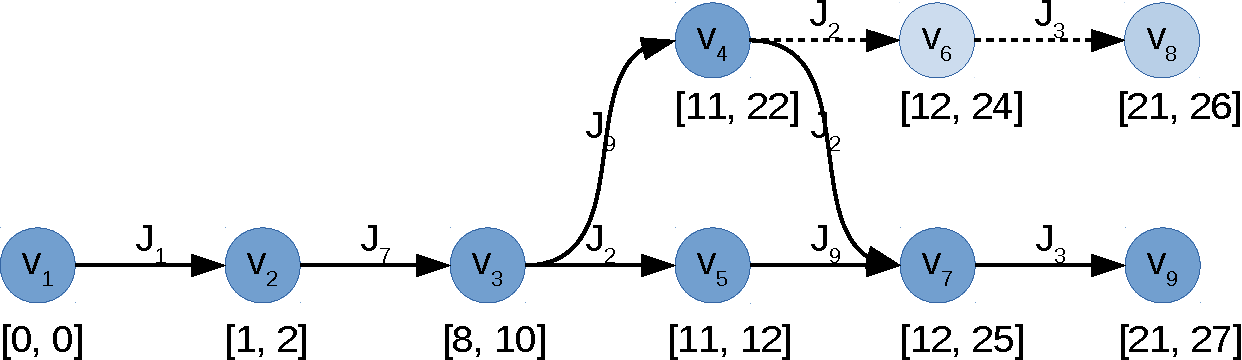
\includegraphics[width=0.8\linewidth]{images/scheduling_graph_merge.pdf}

    \caption{Non-preemptive task-set where $J_7$ finishes 1 time unit earlier, scheduled under
    \acrshort{edf} or \acrshort{rms}}

    \label{fig:scheduling_graph_merge}

\end{figure}

\section{The AER Execution Model}

The \acrfull{aer} execution model was first proposed in \parencite{durrieu_predictable_2014} to
improve performance and predictability while using \acrshort{cots} multi-core processors with shared
and private memory in the avionics industry. It builds on top of the \acrfull{prem} first presented
in \parencite{pellizzoni_predictable_2011} which introduces the idea of dividing tasks into a memory
access phase and an execute phase. Since the bottleneck for utilization in multi-core systems can
become the contention in access to shared memory when introducing an increasing number of cores
\acrshort{aer} focuses on making shared memory access more deterministic and easier to analyse. This
is done by dividing up each task into three distinct parts. The \textbf{acquisition} (A) part reads all
the data necessary for execution of the task such as code and shared variables into the private
memory of the core dedicated for execution. The \textbf{execution} (E) phase then executes the code,
without making any further read or write instructions to the shared memory, operating on local
copies of the shared variables. The \textbf{restitution} (R) phase then writes back all of the acquired
results of the task to the shared memory. Since the A-phase only is allowed to execute before
execution of the task actually starts a pre-requisite of the model is that each core has a separate
private memory, such as a cache or a scratchpad. Since these types of memory often are constrained
in size it puts a limit to how many instructions a task can consist of in addition with the amount
of share variables that is used as they all must fit in the private memory of the core.

The idea of this model is to enable scheduling of the read and write accesses to the shared memory
instead of scheduling the tasks onto cores. Since contention of the shared memory is what limits the
utilization of the cores it is more important to combat this instead of trying to find the optimal
assignment of tasks onto cores since it wont increase utilization anyways. \acrshort{aer} can be
said to employ a \textit{memory-centric} approach to scheduling instead of a \textit{core-centric}
approach that schedulers usually employ. Since no reads and writes to shared memory is allowed
outside of the allocated phases a non-preemptive scheduling algorithm is a pre-requisite for the
\acrfull{aer} model. This model also have the advantage of easier analysis by being more
deterministic. When several cores compete for resources and create congestion which leads to timing
deviations the system model becomes more complex thus harder to analyse. Timing that was calculated
offline, for example the \acrshort{wcet}, may not match reality or require very pessimistic
approximations that exaggerate the timings, both of which decreases the certainty or predictability
of the design and analysis.

The scheduling algorithm proposed in \parencite{durrieu_predictable_2014} to schedule the memory
accesses is a partitioned non-preemptive offline algorithm. The paper \parencite{maia_closer_2016}
further evaluates the \acrshort{aer} model by testing different scheduling algorithms. Instead of
using offline partial scheduling it proposes five different heuristic algorithms under online global
scheduling. These algorithms assign a higher task priority according to period (\acrshort{rms}),
shortest acquisition phase, longest acquisition phase, shortest restitution time and longest
restitution time. It is shown through analysis that the \acrshort{rms} scheduler is far best in
terms of schedulable task sets as their utilization increases. The paper
\parencite{becker_contention-free_2016} explores further ways of scheduling under an \acrshort{aer}
model by proposing a global scheduling algorithm that is shown to only behave 0.5\% worse than an
optimal \acrshort{ilp} algorithm in a fraction of the time.

% AER is an improvement over other models such as proposed by pikeOS which enables all other cores
% to be paused while running critical tasks on a single core.


\section{Related Work}

The most important paper to discuss is \parencite{nasri_response-time_2018} which provides a
state-of-the-art schedulability analysis method for non-preemptive static-priority tasks sets under global
scheduling. The analysis is sufficient for multi-core systems and a corresponding precise method for
uni-core systems by the same authors is presented in \parencite{nasri_exact_2017}. The paper is
explained in detail in section \ref{subsec:artafnpjsug}. Since the thesis builds on top of the
concept of the \acrshort{aer} model it is necessary to be familiar with the paper
\parencite{durrieu_predictable_2014} which was the first to present this model and presents an
offline non-preemptive partitioned scheduling algorithm to schedule the memory accesses. The idea to divide
up tasks into distinct execution phases is not a novel one as \acrshort{aer} builds on top of the
\acrshort{prem} which divides up tasks into a read and execute phase for single-core system and was
first presented in \parencite{pellizzoni_predictable_2011}. The \acrshort{aer} model is
further explored in \parencite{maia_closer_2016} which presents five new global non-preemptive
online scheduling algorithms where the most successful assigns priorities to tasks based on their
period in the same way \acrshort{rms} works. It is also shown to be able to schedule tasks sets that
would otherwise not be schedulable under global \acrshort{edf} due to congestion.

%TODO: Mention that this does no take into the account the deadline of the R-phase.
%TODO: Maybe keep all related work covering scheduling analysis in a new subsection
Some work on analysing have been done on analysing the schedulability of algorithms developed around
\acrshort{prem} such as \parencite{alhammad_schedulability_2014} which builds on the idea of a
problem window from \parencite{baker_multiprocessor_2003}. This idea presents an analysis method for
\acrshort{edf} and \acrshort{dms} on multi-core processors and defines the problem window as the
time interval between the release time and deadline of a certain task $ \tau_i $. The method works
by contradiction where the task is assumed to miss its deadline within the window. An upper bound $
UB(\psi_i) $ of the interference in the timing window $ \psi_i $ is defined as the maximum amount of
utilization that the task set $ \Gamma $ could possibly generate inside the timing window. The lower
bound $ LB(\psi_i) $ is then defined as the demand required on the problem window for $ \tau_i $ to
miss its deadline. The condition $ UB(\psi_i) \le LB(\psi_i) $ then defines a sufficient
schedulability condition for work-conserving schedulers if it is shown to hold for every task in the
task set. The paper extends the \acrshort{prem} to a multi-core scheduler and called
\acrshort{gprem} which is a global static-priority scheduler. This scheduler is shown to, on
average, schedule more task sets than a baseline global round robin scheduler that does not account
contention for all cases that was tried. The different cases were different utilization, different
period ranges, different tasks per core and different number of cores.

The paper \parencite{maia_schedulability_2017} specifically tackles analysis for the \acrshort{aer}
model for multi-core systems by using the theory of a problem windows but applying it in a
bus-centric way. The idea is that by doing analysis of the scheduling of bus accesses instead of the
cores it becomes a single-core problem as only one core can access the bus at a time.  Instead of
checking for an upper bound of the interference that tasks create on cores the method describes a
way to find the upper bound of the interference on the bus created by the other tasks. A bus hole is
defined as "\textit{A bus hole is an interval of time, within the problem window, where all m cores
are busy executing E-phases}" \parencite{maia_schedulability_2017}. The amount of time within all
the bus holes inside the problem window must be enough for the task being examined to schedule its A
and R phases to be able to meet its deadline. The paper describes a method that can compute an upper
bound on the holes in the problem window in pseudo-polynomial time.

The paper \parencite{becker_contention-free_2016} makes an effort to adapt the \acrshort{aer} model
to real applications in the automotive domain by providing a general framework that is also applied
to the physical platform Kalray MPPA-256. It consists of 16 compute clusters that contain 16
processing elements and 16 banks of shared parallel memory each. The concept builds on top of the
\acrshort{autosar} architecture for automotive \acrshort{ecu}'s where the smallest unit of execution
is known as a runnable. Runnables communicate with each other through variables called labels. For
each compute cluster one memory bank is reserved as the shared memory which stores all of the
labels, thus referred to as the label bank. The remaining 15 memory bank are then each assigned as a
private memory to a unique processing element. The runnables running on the processing units are
then executing under the \acrshort{aer} model. A scheduler is then presented to schedule the memory
access phases of the runnables to battle congestion. The scheduling algorithm is said to be a
\textit{memory-centric heuristic} as it schedules the A and R phases on the memory as opposed to a
\textit{core-centric heuristic} that schedules tasks onto cores.

% - autosar, labels, runnables
% - physical hardware platform (MANY-core)
% - scheduler

\subsection{A Response-Time Analysis for Non-Preemptive Job Sets under Global
Scheduling}\label{subsec:artafnpjsug}

%TODO: Mention it requires static-priority assignment
The paper \parencite{nasri_response-time_2018} is the most relevant work for this thesis. It
presents a state-of-the art analysis methods for non-preemptive multi-processor global scheduling.
The method gives a sufficient condition for schedulability. The input is a set of jobs consisting of
their ID, deadline, priority, earliest release time, latest release time, \acrshort{wcet} and
\acrshort{bcet}.  The output then tells whether or not the input is schedulable. The basic idea of
the analysis is to enumerate all of possible combinations of \acrshort{wcet}, \acrshort{bcet} and
release jitter but as not to blow up computation time or memory try to be clever about it. This is
basically done by removing all duplicates of schedules that lead to the same ordering of start times
of the jobs.

The implementation of the analysis works by progressively building a tree graph where each edge
represents a scheduling decision in the form of a specific job assigned to a specific core. The root
node represents the start of scheduling when the first job is available, usually at time zero. 
If two jobs are available simultaneously they will be represented as two different edges in the graph
stemming from the same vertex, even if they are scheduled at the same time instance. Each node
represents a state in time of the schedule and contains information about the interval between the
earliest possible availability and latest possible availability of each core (the time at which a
core is ready to accept a new job) in
system. The root node represents time zero in the schedule at which no job yet has been assigned to
any core. 

The tree graph is built progressively by iterating the algorithm through three different phases.
The expansion phase selects the shortest path from the root to a leaf node and makes a scheduling
decisions (assignment of ready job onto vacant core) and creates its corresponding edge. A unique
edge is created for each core that the job may be assigned to. Each assignment leads to a certain
state of the schedule represented by an added leaf node. The fast-forward phase then progresses 
time until the next scheduling decision is to be made (a core has become vacant). The merge phase is
the part where the analysis is clever by trying to minimize the search space of the tree. Paths that
have scheduled the same job sets in different order but have the same timing values will lead to
identical sub-trees in the future. Because of this it is only necessary to continue evaluation from
one of the nodes effectively making it so that the nodes can be \textit{merged}.


\subsection{An Exact and Sustainable Analysis of Non-Preemptive Scheduling}


\subsection{Contention-Free Execution of Automotive Applications on a Clustered Many-Core Platform}



\chapter{<The work> Use a self-explaining title}

\section{Task model} \label{sec:work_task_model}

The term \textit{schedulability window} is used to refer to the time interval within which a task is
able to be scheduled to not miss its deadline. 

A problem arises when the interval between the worst-case finish time of the A-phase and the
best-case release time of the R-phase is less than the \acrshort{wcet} of the E-phase. The analysis
can't make the guarantee that the interval between the finish time of the A-phase and the start time
of the R-phase is sufficient for the E-phase to finish its execution. The problem becomes even worse
as the schedulability windows of the A-phase and R-phase overlaps as the analysis doesn't handle any
precedence constraints among jobs. This means that it would be possible for and R-phase to be
scheduled before the A-phase belonging to the same job.

It is a property of the model that A-phases must always precede the R-phase belonging to the same
task. It also becomes more complicated than a simple precedence constraint as the analysis must
leave sufficient time between the finish time of the A-phase and the start time of the R-phase for
the E-phase to finish execution. This can be circumvented by constraining the model. The interval
from release to deadline of a job can be divided into three distinct intervals that can be thought of
as sub-windows of the schedulability window of a task. These windows are referred to as the
acquisition-window, the execution-phase and the restitution-window. The execution-phase is still
referred to the same as it will have a static placement within the scheduling window as opposite to
the other two phases which will be schedulable anywhere within their window. This idea is
illustrated in figure \ref{fig:aer_window_model}.


\begin{figure}

    \centering

    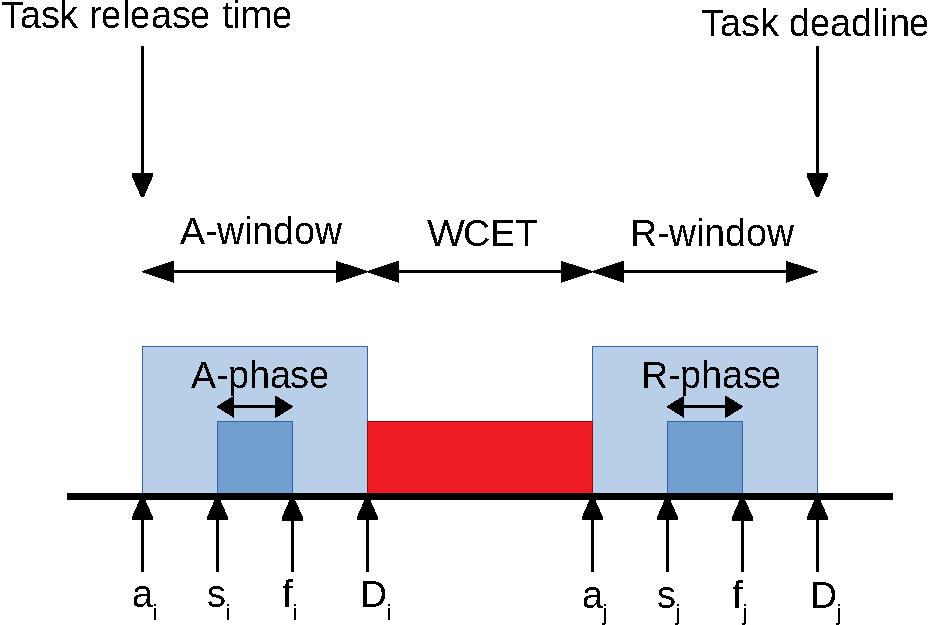
\includegraphics[width=0.8\linewidth]{images/aer_window_model.pdf}

    \caption{The AER window model}

    \label{fig:aer_window_model}

\end{figure}


The task is divided into two separate jobs, one job, denoted $J^{A}$, represents the
acquisition-phase and the other job, denoted $J^{R}$, representing the restitution-phase both being
separated by the \acrshort{wcet} of the task. Each individual job can the be scheduled representing
the memory access and the restitution-phase does not have to worry if the acquisition-phase and the
execution-phase have yet to finish execution as a property of the model is that the
restitution-phase will never be released before the execution-phase is guaranteed to have finished
even in the worst-case. One interesting thing of the model is to chose the \textbf{window-ratio}
between the acquisition-window and the restitution-window as they necessarily don't have to be of
the same size. This will be explored further during benchmarking which is explained in chapter
\ref{sec:benchmarking}.


It quickly becomes obvious however that the model has some disadvantages. The most obvious one being
that the core which the task is assigned to might idle for a long time when the acquisition and
execution phases finish executing, especially in the best case, as the restitution phase is yet to
be released. Another problem is that the number of tasks with the same period can never be larger
than the amount of physical cores as the task set would never be schedulable then. Imagine all but
one task of the same periods and same window-ratio being assigned cores at the same time such that
all cores are busy. The occupied cores would then be busy until the restitution-phases are finished
executing, at which the acquisition-phases are all guaranteed to have had their deadlines passed,
thus the unassigned task will miss its deadline.


\section{Idle-time Insertion Policy} \label{sec:iip}

% TODO: Explain IIP in theoretical framework instead?
% TODO: Mention IIP-eligibility

% TODO: Move to background "work-conserving vs. non-work-conserving"
Imagining a non-preemptive scheduler and a long-running, low-priority task with a deadline far into
the future that has just been released and is about to be scheduled onto a core. If a
higher-priority task with a short deadline is released just after the first tasks has been scheduled
it might miss its deadline as the core wont be available for a long time. In this instance it could
prove beneficial for the schedulability of the task set to leave a core idle even when there is work
to be completed to wait for a higher priority task to be released. 

For the \acrshort{iip} to make a decision it is provided with three pieces of information. First
the job-set of jobs that have previously been scheduled and are finished, second it is provided the
job that just has been released and is to be scheduled, thirdly it is provided the present time at
which the released job is to be scheduled.  The policy then returns a true or false value
representing if the provided job is schedulable at that time. The functionality of an \acrshort{iip}
can thus be described by algorithm \ref{algo:iip_eligibility}, inspired by
\parencite{nasri_exact_2017}.

\begin{algorithm}
    \caption{IIP eligibility}
    \label{algo:iip_eligibility}
    \begin{algorithmic}[1]
        \State $J_i\gets Highest\ priority\ released\ job$
        \If {$aer\_iip(J_i, t, \mathcal{J}^S, c) = true$}
        \Comment{Algorithm \ref{algo:aer_iip}}
            \State $schedule(J_i)$
        \Else
            \State $idle\_processor()$
        \EndIf
    \end{algorithmic}
\end{algorithm}

\begin{algorithm}
    \caption{AER IIP}
    \label{algo:aer_iip}
    \begin{algorithmic}[1]
        \Function{$aer_iip$}{$J_i, t, \mathcal{J}^S, c$}
            \If{$is\_restitution(J_i)$}
                \State \Return true
            \Else
                \If{$free\_cores(\mathcal{J}^S, c) > 0$}
                \Comment {Algorithm \ref{algo:available_cores}}
                    \State \Return $true$
                \Else
                    \State \Return $false$
                \EndIf
            \EndIf
        \EndFunction
    \end{algorithmic}
\end{algorithm}

\begin{algorithm}
    \caption{Available Cores}
    \label{algo:available_cores}
    \begin{algorithmic}[1]
        \Function{$free\_cores$}{$\mathcal{J}^S, c$}
            \State $sum\gets 0$
            \ForAll{$J \in \mathcal{J}^S$}
                \If {$is\_restitution(J)$}
                    \State $sum\gets sum-1$
                \ElsIf{$is\_acquisition(J)$}
                    \State $sum\gets sum+1$
                \EndIf
            \EndFor
            \State \Return $c - sum$
        \EndFunction
    \end{algorithmic}
\end{algorithm}


The scheduling analysis tool was extended by implementing a custom \acrshort{iip}. Scheduling tasks
using a memory-centric approach can be described as a non-work-conserving scheduler as cores might be
left idle, even when there is work to be done, if the memory is busy during the release of a task. 


\subsection{Proof}

No changes have been done to the original algorithm presented in \parencite{nasri_exact_2017} which
also provides the proofs for it. Since the original algorithm allows for any \acrshort{iip} to be
plugged in proof will be given for the developed \acrshort{iip}. The policy is invoked each time a
job is to be scheduled as to see if the job is available for scheduling at that time or if the
processor should idle until a higher priority job is released, when the \acrshort{iip} will be
called upon again.

% 3 Cases:
%   - R-phase
%   - A-phase available core
%   - A-phase no available core
%       - New top Priority
%       - Other released, non-scheduled A-phase, has higher priority (IIP not invoked)
%
% Premises:
%   - R-phases are always higher priority than A-phases
%   - Any job can not execute without being assigned to a core
%


% Write proof of correctness

\subsection{Testing}

Testing of software is always important do make sure it exhibits the desired behaviour. As the
software developed within the thesis was an extension to already existing software the testing
focuses only on the extension. The existing software has also been tested extensively using the c++
testing framework called doctest. To test the developed software a much more basic approach was used
were well defined input was manually fed as input to the program and checking that the output
corresponded to the expected outputs. Debugging was also used to check that the internal control
flow was as expected. The input was chosen to represent both the average-case and edge-cases to
increase coverage and the chance to catch undesired behaviour and bugs in the code.


\section{Scheduling algorithms} \label{sec:scheduling_algorithms}

As the described analysis takes a task set to see if they make a feasible schedule by
scheduling the jobs according to predefined priorities they have to be assigned in some
deterministic way. The analysis does not put constraint on how to assign priorities, only that they
are scheduled non-preemptively. There are several well-defined scheduling algorithms that can be
used, but because of the novelty of the task model it is also interesting to explore
if new scheduling algorithms could better exploit the nature of the task model and compare their
results to existing algorithms.

There are several interesting ways to prioritise the jobs. Existing scheduling algorithms
\acrshort{edf} and \acrshort{rms} can be used. Note however that using \acrshort{rms} for a job
set using periods defined by the \acrshort{autosar} standard has its limitations. For a large task
set a lot of tasks will have the same period, thus their jobs will have the same priority, so it is
of interest to further prioritise the jobs which shares the same period according to some
tie-breaker. The implementation of \acrshort{np}-test tie-brakes priorities based on task-id and
job-id where lower id's are given higher priorities. A more  idea is to prioritize jobs within their
period group according to their utilization as it might prove to increase the schedulability. To
test this seven different scheduling algorithms are proposed and will be used during benchmarking.

\begin{itemize}
    \item \textbf{\acrshort{edf}} - Eearliest Deadline First
    \item \textbf{\acrshort{lulp}} - Low utilization and low period have the highest priority
    \item \textbf{\acrshort{luhp}} - Low utilization and high period have the highest priority
    \item \textbf{\acrshort{hulp}} - High utilization and low period have the highest priority
    \item \textbf{\acrshort{huhp}} - High utilization and high period have the highest priority
    \item \textbf{\acrshort{lu}} - Low utilization have the highest priority (period is ignored)
    \item \textbf{\acrshort{hu}} - High utilization have the highest priority (period is ignored)
\end{itemize}

\begin{figure}

    \centering

    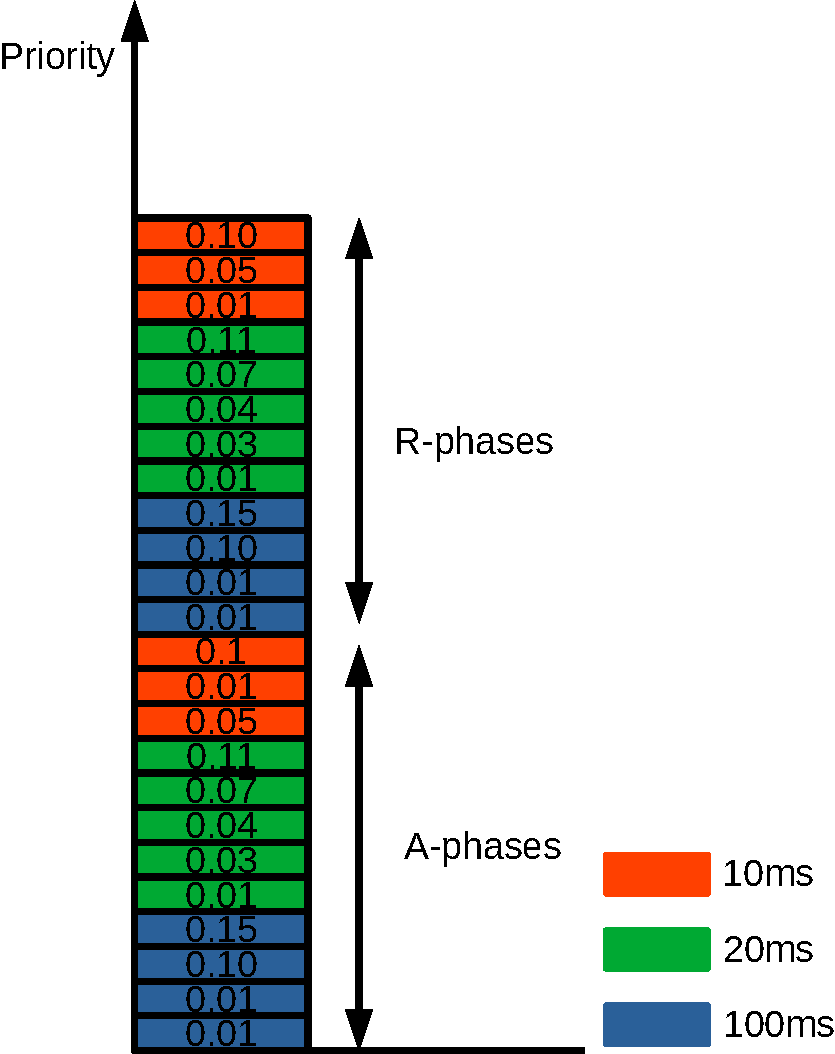
\includegraphics[width=0.8\linewidth]{images/scheduling_priorities.pdf}

    \caption{Priorities assigned according to a HULP scheduler with utilization written on each task}

    \label{fig:scheduling_priorities}

\end{figure}

The general concept of prioritization in this manner is depicted in figure
\ref{fig:scheduling_priorities} which describes how jobs would be prioritized according to
\acrshort{hulp}. The priorities are ordered along the x-axis where higher priorities are higher up
and a job is depicted by a box.
It is important to remember that all of the restitution-jobs must have a higher priority than all of
the acquisition-jobs as described in section \ref{sec:iip}. As can be seen in the figure the highest
priority is given to the restitution-jobs with the lowest periods (10ms) colored orange. Within the
period the jobs are then prioritized according to their utilization which is depicted by the number
on the job. 


% RMS isn't a good choice as there are many tasks with the same period, and they will just be
% scheduled according to task-id on the task-level


\section{Benchmarking}\label{sec:benchmarking}

To benchmark the \acrshort{iip} job sets have to be generated that conform to
the \acrshort{aer} model as well as conform to the input restrictions of the
analysis tool. The input to the analysis is in the form of a \acrfull{csv}
file. It is a plain-text file where each new line holds a unique job to be
scheduled where the columns in the row represents attributes separated by
commas. The columns expected by the analysis tools are as follows.

\begin{itemize}
    \item \textbf{Task ID} - The ID of the belonging task
    \item \textbf{Job ID} - Its unique ID
    \item \textbf{Arrival min} - Its earliest release time
    \item \textbf{Arrival max} - Its latest release time
    \item \textbf{Cost min} - Its \acrshort{wcet}
    \item \textbf{Cost max} - Its \acrshort{bcet}
    \item \textbf{Deadline} - The time at which the job must have finished execution
    \item \textbf{Priority} - Its priority in relation to the other jobs
\end{itemize}


\begin{figure}

    \centering

    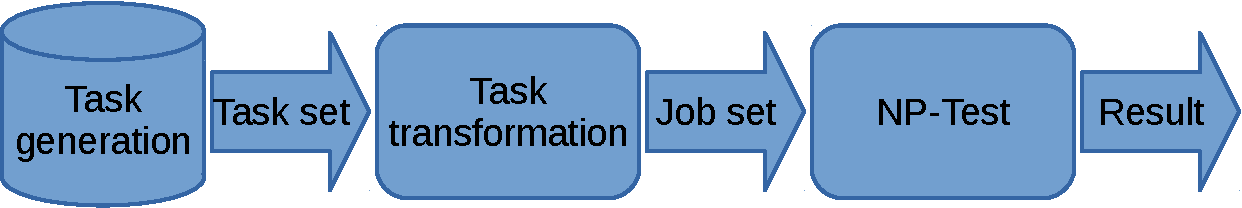
\includegraphics[width=0.8\linewidth]{images/benchmark_toolchain.pdf}

    \caption{Priorities assigned according to a HULP scheduler with utilization written on each task}

    \label{fig:benchmark_toolchain}

\end{figure}


Thus all of these properties must be properly generated in order to perform benchmarks. One option
would be to just randomize everything, but this would not be very reflective of any real systems as
they are usual more formal. Since a lot of the benchmarking will explore how the analysis tool
performs under different utilizations a good starting point would be to explore how tasks sets can
be generated given the total desired utilization and the desired amount of tasks. Generating the
amount of tasks to be constant is important, as tasks sets of different sizes but with the same
utilizations have been shown to have different average
schedulability\parencite{sebestyen_simulation-based_2012} on average for many schedulers and could
thus have an effect on the results. The amount of tasks generated for a set utilization should
therefor carefully be put into consideration. 


\subsection{Task generation}

The paper \parencite{bini_measuring_2005} goes into great detail explaining some of the common pitfalls
when creating good task sets for benchmarking. It also presents the \textbf{Uunifast} algorithm,
which is an $O(n)$ algorithm used to create sets of utilization values. The algorithm takes two
inputs, the size of the set to be created and the total utilization sum of all elements in the sets.
Once the output of the algorithm has been acquired it becomes a more trivial task to generate task
sets by using the given utilizations.

After the utilizations have been generated the next step would to create the tasks. This can now be
approached from two different directions. Either the periods of the tasks can be generated, and from
them the execution times using the already generated utilizations. Or the process can be reversed
and the execution times can be generated first and then the periods from them based on the
utilization set. In addition, we want to create the task set to be as reflective of reality as
possible. Testing a scheduler on tasks sets that doesn't represent reality can be interesting, but
showing that this is something that can be used in real systems is by far more interesting.

Since the majority of interest in the \acrshort{aer} model lies within the automotive and avionics
sector the task set should cohere to the standards and practices to these industries in some way.
However large companies tend to be very secretive of their work but luckily there is a standard
within the automotive industry called \acrshort{autosar} when developing embedded systems that has
been agreed upon to make it easier for cooperation between corporations. According to the
\acrshort{autosar} standard, the period intervals for periodic tasks must be selected from nine
predefined intervals which are 1, 2, 5, 10, 20, 50, 100, 200, 1000 milliseconds. The standard also
defines aperiodic tasks as either being driven by interrupts, or being angle-synchronous, which
means that they are triggered by a certain angle of the crank-shaft, making the period a function of
the rotations-per-minute of the crankshaft. Even though aperiodic tasks are accepted by the analysis
tool they are outside of the scope of this thesis.

%TODO: Explain the choice to not use the 1000ms period during experiments
Since a set of predefined periods are given the execution times of the tasks can easily be generated
from randomising a period and pairing it with a random utilization from the set created by the
uunifast algorithm. However, the probability distribution for the periods might not be uniform for a
real life system which could be put into consideration when choosing the period. Luckily a research
group at Bosch have released benchmarking data from real world automotive systems to be used for
free by anyone in the paper "Real World Automotive Benchmarks For Free"\parencite{kramer_real_2015}.
The data has been extracted from a real-world application to a point where it doesn't doesn't give
away any \acrshort{ip}-critical information about the actual application. The actual distribution
for the periods are given in table \ref{tab:period_distribution}. Since we do not consider
angle-synchronous tasks in this thesis the extra 15\% is simply ignored and the remaining
percentages are scaled such that their sum equals 100\%. 

\begin{table}
    \centering
    \begin{tabular}{| c | c |} 
        \hline
        Period & Probability \\
        \hline
        1 ms & 3\% \\
        \hline
        2 ms & 2\% \\
        \hline
        5 ms & 2\% \\
        \hline
        10 ms & 25\% \\
        \hline
        20 ms & 25\% \\
        \hline
        50 ms & 3\% \\
        \hline
        100 ms & 20\% \\
        \hline
        200 ms & 1\% \\
        \hline
        1000 ms & 4\% \\
        \hline
        Angle-synchronous & 15\% \\
        \hline
    \end{tabular}
    \caption{Distribution of periods within a real \acrshort{autosar} system. Taken from \parencite{kramer_real_2015}}
    \label{tab:period_distribution}
\end{table}

After pairing a utilization with a period to create the tasks execution time the question remains
how to decide the \acrshort{wcet} and \acrshort{bcet}. Even though the free benchmarks from Bosch
offers a way to generate these from the average execution time and it is accepted by the
\acrshort{np}-test it does not provide any additional benefit to the benchmark. This becomes more
clear in chapter \ref{sub:task_transformation} but the short reason is that only the \acrshort{wcet}
is used when creating the job set and setting it to something different than what was generated by
the uunifast algorithm will change the total utilization of the task set, which is undesirable.

The execution times of the \acrshort{a}-phase and \acrshort{r}-phase is functions of the size of
the data read and written to the memory during each phase which can be very deterministic when we
assume no cache and don't allow the phases to be preempted. The question remains what size to pick
for the phases and it is not trivial. The paper "Scheduling Multi-Rate Real-Time Applications on
Clustered Many-Core Architectures with Memory Constraints"\parencite{becker_scheduling_2018} contains
information about the execution times of the acquisition and restitution phases of 18 different
tasks in an engine management system in a car. These could be used to make approximations of the
ratios between the execution times of the three different phases. It is however of interest to
benchmark how the schedulability of the job sets is affected by varying the ratios between the three
phases. These ratios are thus instead provided during benchmarking as an input to the task
generator.

The ratios determine how much of the total execution phase, which was determined earlier by the
utilization and period, should be allocated to the \acrshort{a} and the \acrshort{r} phases, where
differing ratios between them is possible. This mean that they "steal" execution time from the
\acrshort{e} phase. This is in order to not change the total utilization of the task set in any way.

The \acrshort{np}-test accepts the release-time to be defined as an interval in case of jitter in
the system. This is not used in benchmarking and the worst-case release time is thus defined to be
the same as the best-case release time, which is right at the beginning of each new period for every
task.

Priorities are assigned by a scheduler according to some property of the task such as \acrshort{edf}
assigns priorities based on the deadlines.

%TODO: Mention that even though one could create a much more accurate task set using the information
%given in free benchmarks it would be hard to adhere it to a set total utilization and it would be
%a large enough scope for a thesis of its own.

\subsection{Task transformation} \label{sub:task_transformation}

As the task sets generated thus far does not hold the information that is required by the analysis
tool, explained in \ref{sec:benchmarking}, they have to be transformed into a regular job-set. This
job-set does not hold any explicit data that would separate it from a regular job-set even though it
actually represents tasks under the \acrshort{aer} model, all this information is instead implicit.
This can be done as long as the task generation phase provides sufficient information about the
tasks in its output. The necessary information is as follows.

\begin{itemize}
    \item \textbf{Task ID} - The tasks ID
    \item \textbf{Arrival min} - The earliest relative release time
    \item \textbf{Arrival max} - The latest relative release time
    \item \textbf{Computation min} - The \acrshort{bcet} of the execution-phase
    \item \textbf{Computation max} - The \acrshort{wcet} of the execution-phase
    \item \textbf{Acquisition max} - The \acrshort{wcet} of the acquisition-phase
    \item \textbf{Restitution max} - The \acrshort{wcet} of the restitution-phase
    \item \textbf{Deadline} - The relative deadline
    \item \textbf{Priority} - The priority relative to other tasks in the set
    \item \textbf{Period} - The period 
\end{itemize}

So all of this information about a task set is then to be transformed into a job set represented by
the characteristics given in chapter \ref{sec:benchmarking} to be accepted as input to the
\acrshort{np}-test. The basic idea in transforming the \acrshort{aer}-modeled task set into a
regular job set is to make the acquisition- and restitution-phases of each period into individual
jobs. Although the execution-phase is not turned into its own job it still holds vital information.
The reason is that the jobs are to be scheduled around memory-accesses, and the whole point of the
\acrshort{aer}-model is that the execution-phase holds no memory-accesses to shared memory and as
such doesn't have to directly be taken into account of the scheduler. The way the execution-phase
will be used is to represent the constraint that the interval between the deadline of the
acquisition-phase and the earliest release time of the restitution phase must be that of at least
the \acrshort{wcet} of the execution-phase. This ensure that the acquisition job is not scheduled
until the execution-phase is guaranteed to have finished. 


\begin{algorithm}
    \caption{Task transformation}
    \label{algo:task_transformation}
    \begin{algorithmic}[1]

        
        \renewcommand{\algorithmicrequire}{\textbf{Input:}}
        \Require $W \in [0, 1]$: ratio between A and R windows, $\Gamma$: \acrshort{aer} task set
        

        \State $hyperperiod \gets 0$
        \ForAll{$\tau \in \Gamma$}
            \Comment Find the hyperperiod
            \State $hyperperiod \gets lcm(hyperperiod, \tau_T)$
        \EndFor


        \State $id \gets 1$
        \ForAll{$\tau \in \Gamma$}
            \Comment Create jobs for each task in the task set

            \State $window\_size \gets \tau_{D} - \tau_{r^{min}} - \tau_{C^{max}}$ 

            \For{$i \gets 0, hyperperiod/\tau_T$}
                \State $t \gets i * \tau_T$
                \Comment Absolute time for the period

                \State //Create the acquisition job
                \State $J^{A}_{id} \gets id$
                \State $id \gets id + 1$
                \State $J^{A}_{task\_id} \gets \tau_{id}$
                \State $J^{A}_{r^{min}} \gets t + \tau_{r^{min}}$
                \State $J^{A}_{r^{max}} \gets t + \tau_{r^{max}}$
                \State $J^{A}_{C^{min}} \gets \tau_{acquisition}$
                \State $J^{A}_{C^{max}} \gets \tau_{acquisition}$
                \State $J^{A}_d \gets t + \left \lceil{W * window\_size}\right \rceil $
                
                \State //Create the restitution job
                \State $J^{R}_{id} \gets id$
                \State $id \gets id + 1$
                \State $J^{R}_{task\_id} \gets \tau_{id}$
                \State $J^{R}_{r^{min}} \gets J^{A}_d + \tau_{C^{max}}$
                \State $J^{R}_{r^{max}} \gets J^{A}_d + \tau_{C^{max}}$
                \State $J^{R}_{C^{min}} \gets \tau_{restitution}$
                \State $J^{R}_{C^{max}} \gets \tau_{restitution}$
                \State $J^{R}_d \gets t + \tau_D $

                \State $\mathcal{J} \gets \mathcal{J} \cup \{J^A\} \cup \{J^R\}$
                \Comment Add created jobs to the job set
            \EndFor
        \EndFor
        \State $assign\_priorities(\mathcal{J})$
        \Comment Assigning priorities relies on all jobs having been created

    \end{algorithmic}
\end{algorithm}


The jobs are created according to algorithm \ref{algo:task_transformation}. Since a schedule is
bound to repeat itself after one hyperperiod it is sufficient to test the schedulability during this
interval. Thus the algorithm first finds the hyperperiod of the task set by finding the
least-common-multiple of all the periods. It is then sufficient to create the jobs that are released
within the hyperperiod, placing an upper-bound on their release times. This ensures that the
task-transformation will terminate. The jobs are then created from one task at a time until jobs for
all tasks have been created. The tasks \textbf{window size} is defined as the total time of the
acquisition-window plus the restitution-window. It is used in conjunction with the window ratio to
calculate the actual sizes of the windows. Since the \acrshort{np}-test requires absolute time
(as opposed to relative time which is relative to the start of the period) the start time for each
period is calculated and used to to transform relative time values to absolute ones. This continues
until the hyperperiod is reached at which no more jobs is created for that task. Since all The jobs
are created in pairs of an acquisition-job and a restitution-job where the acquisition-job is
created first and given an odd job-id as required and further explained in section \ref{REF}. Its
release time is then transformed from the tasks relative release time to an absolute release time.
Its worst-time execution time is then assigned according to the execution time of the acquisition
phase in the task. The deadline is then calculated from the window size and the window ratio which
is given as input to the algorithm and transformed to an absolute time. The restitution phase is
then created in a similar manner, but given an even job-id. Its release times are calculated as the
deadline of the acquisition-job plus the \acrshort{wcet} of the execution-phase. The restitution-job
gets its execution time from the execution time of the restitution-phase in the task. The deadline
is then assigned according to the tasks deadline, but transformed into absolute time. When all the
jobs for every task has been created they are all assigned priorities according to the one of the
scheduling algorithms describes in section \ref{sec:scheduling_algorithms}. This is because the
priorities describe a relation between the jobs, thus all the jobs must sometimes be created before
the priorities can be assigned. 


\subsection{Running benchmarks}

As part of benchmarking a set of experiments will be ran to test what effect different input
variables will have on the schedulability. Each variable that will be put into consideration is
shortly described in the rest of this section.

The experiments will be running on a "HP Z210 Workstation" with a quad-core Intel Core i7-2600 CPU
\@3.40GHz and 16 GiB of memory.

The idea of benchmarking is to recognise the dependent and independent variables of the system, make
changes to the independent variables and see what effect they have on the dependent variables. The
dependent variable of most interest is the \textbf{schedulability ratio} which is the ratio between
schedulable task sets and the total amount of task sets. The independent variables are explained in
the following list.

\begin{itemize}

    \item \textbf{Task amount} - The total amount of tasks to be scheduled
    \item \textbf{Core amount} - The amount of cores available for jobs to be scheduled onto.
    \item \textbf{Scheduling algorithm} - The algorithm used to schedule the system. 
    \item \textbf{\acrshort{a}-ratio} - The execution time of the \acrshort{a}-phase as a ratio of
        the tasks utilization.
    \item \textbf{\acrshort{r}-ratio} - The execution time of the \acrshort{r}-phase as a ratio of
        the tasks utilization.
    \item \textbf{Window ratio} - The ratio between the \acrshort{a}-window and \acrshort{r}-window.
    \item \textbf{Utilization} - The total utilization of all tasks summed.

\end{itemize}

%TODO: Explain why the input is chosen the way it will be, 10% a and r cycles, the task amount, the
%core amount etc.

\subsubsection{Core amount}

When changing the core amount it is of interest to see how the schedulability ratio is affected,
especially when the utilization is kept static. Smaller amount of tasks leads to larger execution
times of each task and vise versa, so imagining the bin-packing problem as explained in chapter

\subsubsection{Task amount}

The idea is to use task amount as a variable and see how the schedulability ratio changes as an
effect on how many tasks needs to be scheduled when other variables are 

\subsubsection{Window ratio}

\subsubsection{Scheduling algorithms}




\chapter{<Result> Use a self-explaining title}

\section{Window sizes}

\begin{figure}

    \centering

    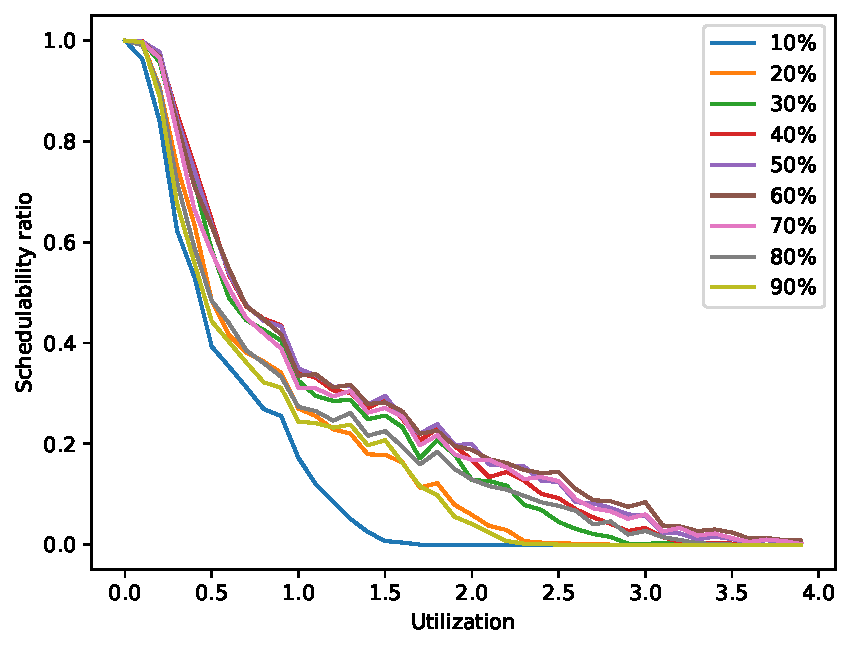
\includegraphics[width=1.0\linewidth]{images/window_ratio.pdf}

    \caption{Priorities assigned according to a HULP scheduler with utilization written on each task}

    \label{fig:window_ratio}

\end{figure}

\begin{figure}

    \centering

    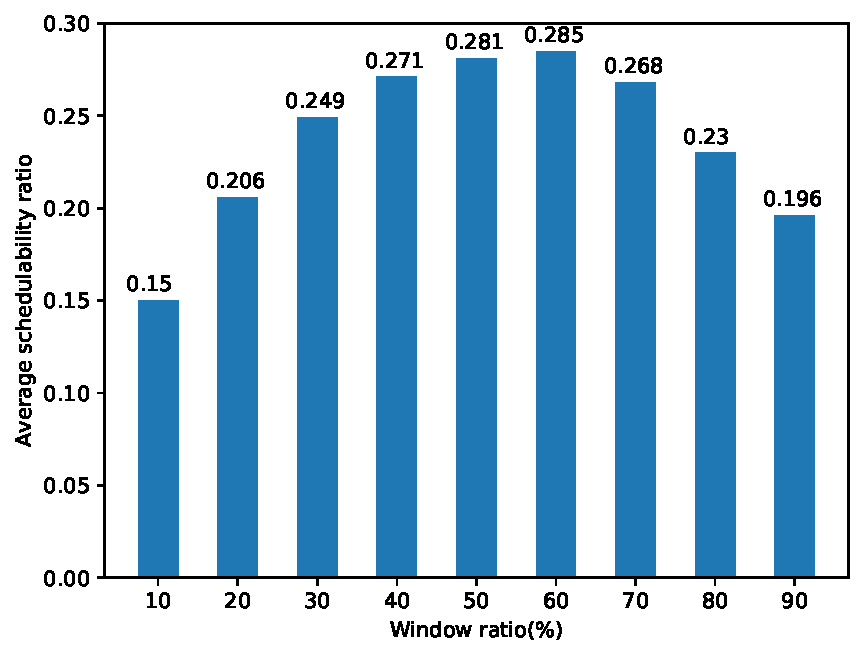
\includegraphics[width=1.0\linewidth]{images/window_ratio_averages.pdf}

    \caption{Priorities assigned according to a HULP scheduler with utilization written on each task}

    \label{fig:window_ratio_averages}

\end{figure}

\section{Task amount}

\begin{figure}

    \centering

    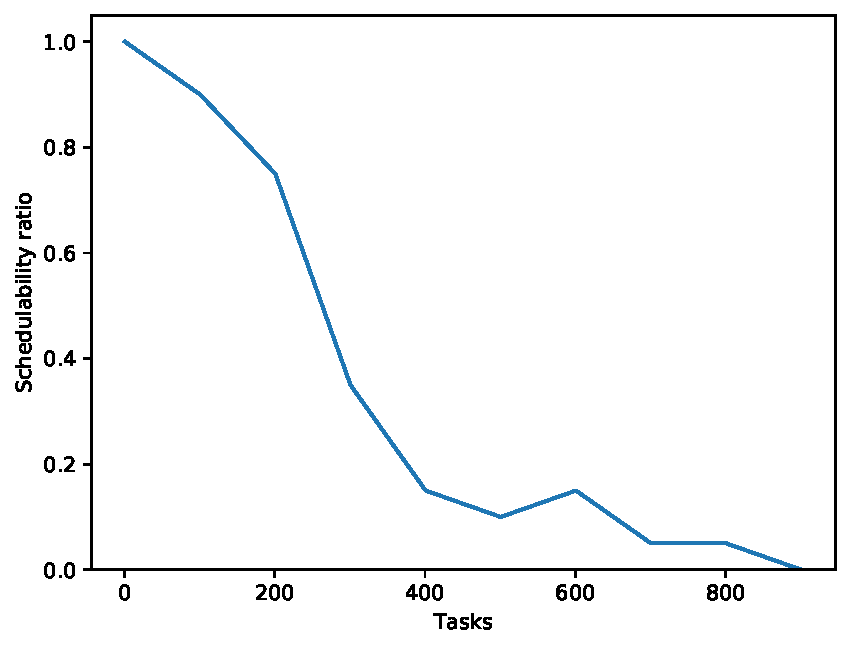
\includegraphics[width=1.0\linewidth]{images/task_amount_2.pdf}

    \caption{Priorities assigned according to a HULP scheduler with utilization written on each task}

    \label{fig:task_amount_2}

\end{figure}

\begin{figure}

    \centering

    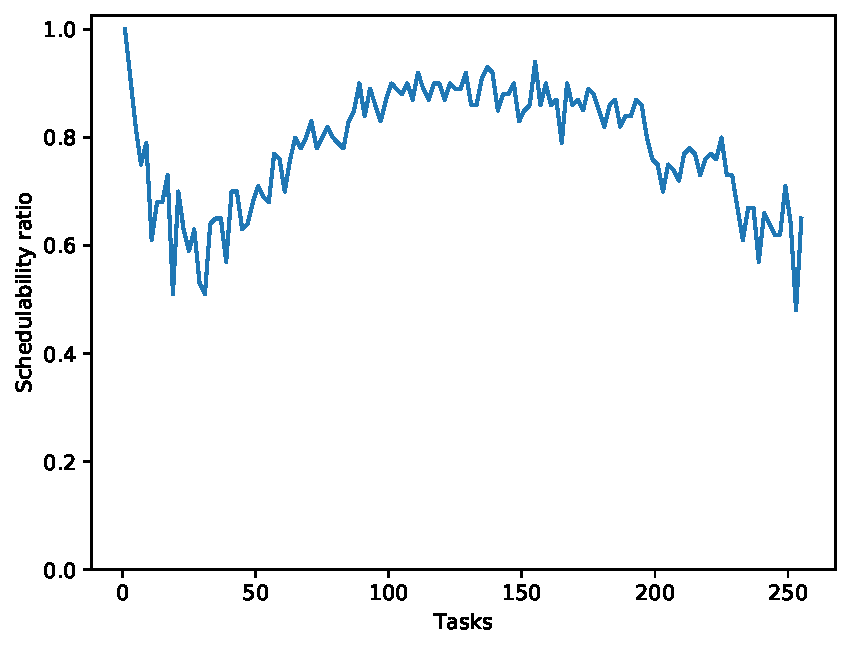
\includegraphics[width=1.0\linewidth]{images/task_amount_1.pdf}

    \caption{Priorities assigned according to a HULP scheduler with utilization written on each task}

    \label{fig:task_amount_1}

\end{figure}

\section{Core amount}

\section{Scheduling algorithms}

\begin{figure}

    \centering

    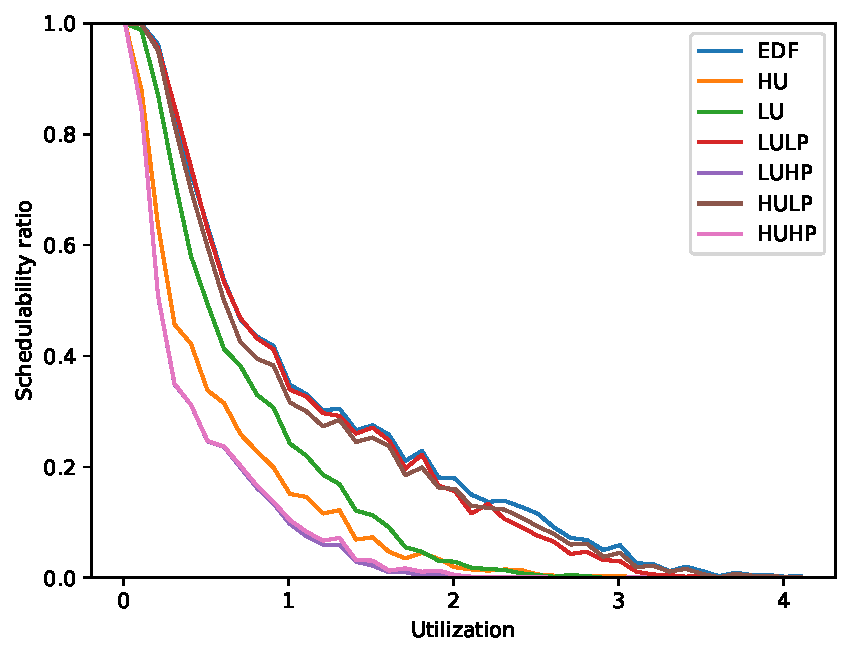
\includegraphics[width=1.0\linewidth]{images/sched_algos.pdf}

    \caption{Priorities assigned according to a HULP scheduler with utilization written on each task}

    \label{fig:sched_algos}

\end{figure}

\section{Reliability}

\section{Validity}

\section{Replicability}


\chapter{<Discussion> Use a self-explaining title}

\section{Scheduling anomaly}

\section{Conclusions}

% Describe how the task model requires that there are not more number of tasks of a given period
% than the total amount of cores in the system, as it will lead to the schedule being not feasible.


\subsection{Future work}

%TODO: Mention that implementing precedence-constraints in the timing analysis makes it such that
%the A and R windows become redundant. Also requires the WCET of E to be added to the A-phase.
    % NOT TRUE. The WCET of E cant be added as it will seem to occupy the memory while its really


% Print the bibliography (and make it appear in the table of contents)
\printbibliography[heading=bibintoc] 

% Start the appendix section
\appendix

% Appendix A
\chapter{Unnecessary Appended Material}


\end{document}
